%%
%% Class homework & solution template for latex
%% Alex Ihler
%%
\documentclass[twoside,11pt]{article}
\usepackage{amsmath,amsfonts,amssymb,amsthm}
\usepackage{graphicx,color}
\usepackage{verbatim,url}
\usepackage{listings}
\usepackage{upquote}
\usepackage[T1]{fontenc}
%\usepackage{lmodern}
\usepackage[scaled]{beramono}
%\usepackage{textcomp}

% Directories for other source files and images
\newcommand{\bibtexdir}{../bib}
\newcommand{\figdir}{fig}

\newcommand{\E}{\mathrm{E}}
\newcommand{\Var}{\mathrm{Var}}
\newcommand{\N}{\mathcal{N}}
\newcommand{\matlab}{{\sc Matlab}\ }

\setlength{\textheight}{9in} \setlength{\textwidth}{6.5in}
\setlength{\oddsidemargin}{-.25in}  % Centers text.
\setlength{\evensidemargin}{-.25in} %
\setlength{\topmargin}{0in} %
\setlength{\headheight}{0in} %
\setlength{\headsep}{0in} %

\renewcommand{\labelenumi}{(\alph{enumi})}
\renewcommand{\labelenumii}{(\arabic{enumii})}

\theoremstyle{definition}
\newtheorem{MatEx}{M{\scriptsize{ATLAB}} Usage Example}

\definecolor{comments}{rgb}{0,.5,0}
\definecolor{backgnd}{rgb}{.95,.95,.95}
\definecolor{string}{rgb}{.2,.2,.2}
\lstset{language=Matlab}
\lstset{basicstyle=\small\ttfamily,
        mathescape=true,
        emptylines=1, showlines=true,
        backgroundcolor=\color{backgnd},
        commentstyle=\color{comments}\ttfamily, %\rmfamily,
        stringstyle=\color{string}\ttfamily,
        keywordstyle=\ttfamily, %\normalfont,
        showstringspaces=false}
\newcommand{\matp}{\mathbf{\gg}}

\begin{document}

\section*{Decision Tree Methods}

We wanted to compare different decision tree methods and see how they perform compared to the other methods. This involved seeing if a single strong learner or multiple weak learners would perform better for this data set. With the weak learners, we decided to see if Random Forests or Gradient Boosting achieved better results. We also wanted to see if boosting the random forests would help also.   

\section*{Single Decision Tree} 

In order to compare the ensemble methods, I wanted a baseline being one decision tree and seeing how much I could optimize the validation error for a single decision tree. The important hyper-parameters for decision trees seem to be minParent and maxDepth. With minParent, it was clear that the ideal value for our data set was $2^9$ from the work we did in Homework 4. The validation error curve clearly showed that $2^9$ was the best value and it began to overfit after that. With maxDepth, the ideal value seemed to have been 15 but I wanted to see if a larger maxDepth would be better or cause the data to overfit. 
\begin{figure}[h]
\centering
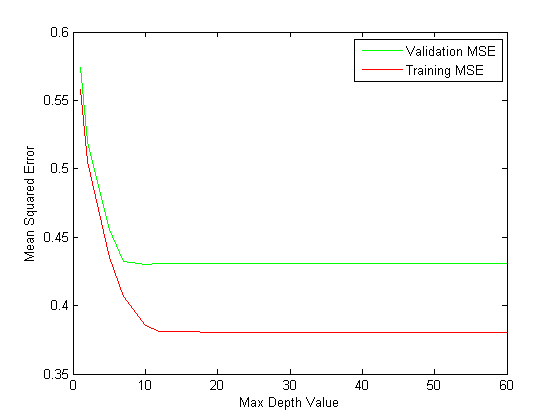
\includegraphics[width=4 in]{maxDepthVersusMSE.png}
\caption{MaxDepth Versus MSE}
\end{figure}
As can be observed, once the maxDepth value reaches 20 or so, the training and validation error stays relatively the same. Since the minParent value was $512$, it is likely that after 20 layers, the decision tree does not have enough data in each node for meaningful splits. In order to verify this, I lowered the minParent value to $32$ to see if we will have the same effect as above, but after a greater number of layers. As it turns out, at 30 layers, the training error stops improving, hence a similar effect is observed. The validation error also stays relatively constant after 30 layers. When you look at the validation error though as a function of maxDepth, it is clear that there is overfitting after about 7 layers. Hence having a low minParent value not only causes more layers to occur but also increases overfitting.  \\
\begin{figure}[h]
\centering
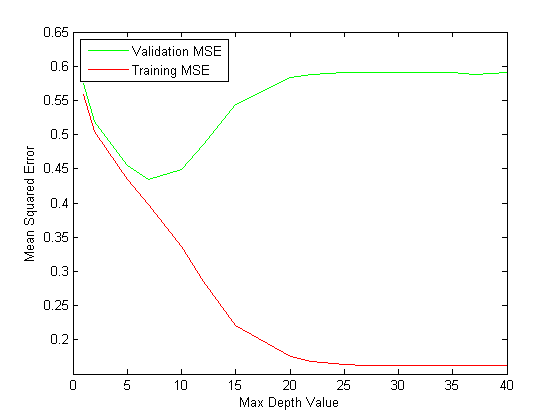
\includegraphics[width=4 in]{maxDepthVersusMSE2.png}
\caption{MaxDepth Versus MSE}
\end{figure}

In the end, the best validation error occcured with minParent equal to 512 and the maxDepth equal to 20, so that is what I used when making the Kaggle data set. The Kaggle MSE ended up being 0.65003. 

\section*{Gradient Boosting}



\section*{Random Forests}



\section*{Gradient Boosted Random Forests}

I wanted to see if a combination of gradient boosting and random forests would work well. I selected a random set of features and then trained their decision trees using gradient boosting. I then averaged together the results. The idea was to use the randomness from random forests but boost each of the trees found. 


\end{document}
